\chapter{Pengelolaan File CSV}

Tujuan pembelajaran pada pertemuan keempat antara lain:
\begin{enumerate}
\item
Mengenal file CSV dan fungsinya 
\item
Mengerti cara memakai library CSV
\item
Mengerti cara memakai library pandas
\item
Mengatasi Error yang terjadi akibat pemakaian library csv dan pandas
\item
Try Except
\end{enumerate}
Tugas dengan cara dikumpulkan dengan pull request ke github dengan menggunakan latex pada repo yang dibuat oleh asisten IRC. Kode program dipisah dalam folder src NPM.py yang berisi praktek dari masing-masing tugas file terpisah sesuai nomor yang kemudian dipanggil menggunakan input listing ke dalam file latex penjelasan atau nomor pengerjaan. Masing masing soal bernilai 5 dengan total nilai 100. Gunakan bahasa yang baku dan bebas plagiat dengan dibuktikan hasil scan plagiarisme. Serta hasil scrinsut dari komputer sendiri, dan kode hasil sendiri. Pengerjaan menggunakan latex dan harus menyertakan file pdf hasil compile pdflatex, jika tidak diskon 50\%.


\section{Pemahaman Teori}
Kerjakan soal berikut ini, masing masing bernilai 5. Untuk hari pertama.
Praktek teori penunjang yang dikerjakan dengan deadline besok jam 4 pagi:
\begin{enumerate}
\item
Apa itu fungsi file csv, jelaskan sejarah dan contoh
\par\textbf{Jawaban}
\par CSV (comma separated value) merupakan sebuah file yang berfungsi untuk mempresentasikan sebuah data. format ini termasuk dalam standar file ASCH. file csv juga dapat diimplementasikan dalam beberapa macam perangkat lunak contohnya ms word,oracle,notepad,MySql,sublime dan lain-lain.
\par \textbf{Contoh :}
\par
      \begin{centering}
          \centering
          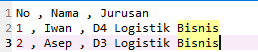
\includegraphics[scale=1]{figures/chapter 4/1.PNG}
      \end{centering}
\item
Aplikasi-aplikasi apa saja yang bisa menciptakan file csv?
\par \textbf{Jawaban}
\begin{itemize}
    \item Microsoft excel
    \item Notepad
    \item Sublime
    \item Google Sheet
    \item dll
\end{itemize}
\item
Jelaskan bagaimana cara menulis dan membaca file csv di excel atau spreadsheet
\par\textbf{Jawaban}
\begin{itemize}
    \item Buka program microsoft excel atau spreadsheet
    \item Buat data pada baris dan kolom
    \item Lalu save as dan memilih save file dengan .csv
\end{itemize}
\item
Jelaskan sejarah library csv
\par\textbf{Jawaban} 
\par Liblary csv mengimplementasikan kelas yang digunakan untuk membaca dan menulis data dalam format .csv. format ini termasuk dalam standar file ASCH. file csv juga dapat diimplementasikan dalam beberapa macam perangkat lunak contohnya ms word,oracle,notepad,MySql,sublime dan lain-lain.
\item
Jelaskan sejarah library pandas
\par\textbf{Jawaban}
\par Liblaryu pandas adalah pustaka perangkat lunak yang ditulis untuk bahasa pemrograman Python untuk manipulasi dan analisis data.
\item
Jelaskan fungsi-fungsi yang terdapat di library csv
\par\textbf{Jawaban}
\begin{itemize}
    \item Reader
    \par Reader berfungsi untuk membaca file .csv
    \item Write
    \par Write berfungsi untuk membuat file .csv
    \item DictReader
    \par Dictreader berfungsi membaca file .csv dari dictionary
    \item DictWriter   
    \par Dictreader berfungsi untuk membaca file .csv dari dictionary
\end{itemize}
\item
Jelaskan fungsi-fungsi yang terdapat di library pandas
\begin{itemize}
    \item read .csv
    \par fungsi ini digunakan untuk membaca atau membuka file .csv
    \item to.csv
    \par fungsi ini digunakan untuk membuat file .csv
\end{itemize}
\end{enumerate}

\section{Ketrampilan Pemrograman}
Kerjakan soal berikut ini, masing masing bernilai 5 untuk hari kedua, lusa jam 4 pagi. Soalnya adalah:

\begin{enumerate}
\item
Buatlah fungsi (file terpisah/library dengan nama NPM\_csv.py) untuk membuka file csv dengan lib csv mode list
\item
Buatlah fungsi (file terpisah/library dengan nama NPM\_csv.py) untuk membuka file csv dengan lib csv mode dictionary
\item
Buatlah fungsi (file terpisah/library dengan nama NPM\_pandas.py) untuk membuka file csv dengan lib pandas mode list
\item
Buatlah fungsi (file terpisah/library dengan nama NPM\_pandas.py) untuk membuka file csv dengan lib pandas mode dictionary
\item
Buat fungsi baru di NPM\_pandas.py untuk mengubah format tanggal menjadi standar dataframe
\item
Buat fungsi baru di NPM\_pandas.py untuk mengubah index kolom
\item
Buat fungsi baru di NPM\_pandas.py untuk mengubah atribut atau nama kolom
\item
Buat program main.py yang menggunakan library NPM\_csv.py yang membuat dan membaca file csv
\item
Buat program main2.py yang menggunakan library NPM\_pandas.py yang membuat dan membaca file csv
\end{enumerate}




\section{Ketrampilan Penanganan Error}
Kerjakan soal berikut ini, masing masing bernilai 5(hari kedua). Bagian Penanganan error dari script python.
\begin{enumerate}
\item
Tuliskan peringatan error yang didapat dari mengerjakan praktek ketiga ini, dan jelaskan cara penanganan error tersebut.
dan Buatlah satu fungsi yang menggunakan gunakan try except untuk menanggulangi error tersebut.
\end{enumerate}



\section{Presentasi Tugas}
Pada pertemuan ini, diadakan dua penilaiain yaitu penilaian untuk tugas mingguan seperti sebelumnya dengan nilai maksimal 100. Kemudian dalam satu minggu kedepan maksimal sebelum waktu mata kuliah kecerdasan buatan. Ada presentasi kematerian dengan nilai presentasi yang terpisah masing-masing 100. Jadi ada tiga komponen penilaiain pada pertemuan ini yaitu :
\begin{enumerate}
	\item tugas minggu hari ini dan besok (maks 100). pada chapter ini
	\item presentasi csv (maks 100). Mempraktekkan kode python dan menjelaskan cara kerjanya.
\end{enumerate}
Waktu presentasi pada jam kerja di IRC. Kriteria penilaian presentasi sangat sederhana, presenter akan ditanyai 20(10 pertanyaan program, 10 pertanyaan teori) pertanyaan tentang pemahamannya menggunakan python untuk kecerdasan buatan. jika presenter tidak bisa menjawab satu pertanyaan asisten maka nilai nol. Jika semua pertanyaan bisa dijawab maka nilai 100. Presentasi bisa diulang apabila gagal, sampai bisa mendapatkan nilai 100 dalam waktu satu minggu kedepan.




